\documentclass[12pt]{article}
\usepackage[utf8]{inputenc}
\usepackage{float}
\usepackage{amsmath}
\usepackage{amssymb}

\usepackage{tikz}
\usetikzlibrary{positioning}

\usepackage[hmargin=3cm,vmargin=6.0cm]{geometry}
%\topmargin=0cm
\topmargin=-2cm
\addtolength{\textheight}{6.5cm}
\addtolength{\textwidth}{2.0cm}
%\setlength{\leftmargin}{-5cm}
\setlength{\oddsidemargin}{0.0cm}
\setlength{\evensidemargin}{0.0cm}

%misc libraries goes here
\usepackage{fitch}

\begin{document}

\section*{Student Information } 
%Write your full name and id number between the colon and newline
%Put one empty space character after colon and before newline
Full Name :  Alperen OVAK\\
Id Number :  2580801\\

% Write your answers below the section tags
\section*{Answer 1}


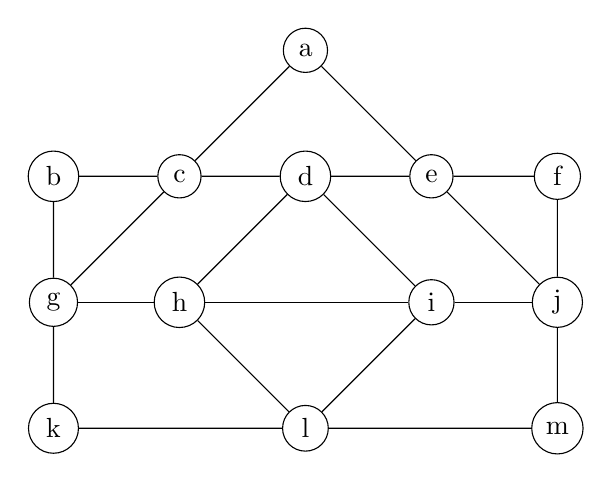
\begin{tikzpicture}[scale=0.8]
    \node[circle,draw] (a) at (0,4) {a};
    \node[circle,draw] (b) at (-4,2) {b};
    \node[circle,draw] (c) at (-2,2) {c};
    \node[circle,draw] (d) at (0,2) {d};
    \node[circle,draw] (e) at (2,2) {e};
    \node[circle,draw] (f) at (4,2) {f};
    \node[circle,draw] (g) at (-4,0) {g};
    \node[circle,draw] (h) at (-2,0) {h};
    \node[circle,draw] (i) at (2,0) {i};
    \node[circle,draw] (j) at (4,0) {j};
    \node[circle,draw] (k) at (-4,-2) {k};
    \node[circle,draw] (l) at (0,-2) {l};
    \node[circle,draw] (m) at (4,-2) {m};
    \draw (a) -- (e) -- (j);
    \draw (a) -- (c) -- (g);
    \draw (d) -- (h) -- (l) -- (i) -- (d);
    \draw (b) -- (g) -- (k);
    \draw (f) -- (j) -- (m);
    \draw (b) -- (c) -- (d) -- (e) -- (f);
    \draw (g) -- (h) -- (i) -- (j);
    \draw (k) -- (l) -- (m);
\end{tikzpicture}

\subsection*{a)}

For a graph to have an Eulerian circuit, each vertex must have an even degree (number of edges incident to it), and the graph must be connected.

From the graph \( G \) provided:

\begin{itemize}
    \item Vertex \( a \) has degree 2.
    \item Vertex \( b \) has degree 2.
    \item Vertex \( c \) has degree 4.
    \item Vertex \( d \) has degree 4.
    \item Vertex \( e \) has degree 4.
    \item Vertex \( f \) has degree 2.
    \item Vertex \( g \) has degree 4.
    \item Vertex \( h \) has degree 4.
    \item Vertex \( i \) has degree 4.
    \item Vertex \( j \) has degree 4.
    \item Vertex \( k \) has degree 2.
    \item Vertex \( l \) has degree 4.
    \item Vertex \( m \) has degree 2.
\end{itemize}

All vertices have even degrees, which means graph \( G \) meets the first criterion.

The graph \( G \) is also connected as you can see in the graph, as we can trace a path from any vertex to any other vertex in the graph by following the edges.

Therefore, graph \( G \) does have an Eulerian circuit.


\subsection*{b)}

For an Eulerian path (that is not a circuit) to exist, the number of vertices which have odd degree must be 0 or 2. Additionally, the graph must be connected.

Since there is no odd degreed vertices, and the graph is connected, we can say that there is an Eulerian path.

\subsection*{c)}

To determine if graph \( G \) has a Hamiltonian circuit, we must find a closed loop that visits each vertex exactly once and returns to the starting vertex.

\textbf{Observations and Analysis:}

\begin{itemize}
    \item \textbf{Vertex Degrees:} The vertices \( a \), \( b \), \( f \), \( k \), and \( m \) have a degree of 2. In a Hamiltonian circuit, we must use all edges connected to vertices of degree 2, entering and exiting each of these vertices.
    
    \item \textbf{Outer Circle Formation:} When we consider the edges connected to vertices of degree 2 and ensure that we enter and exit each of these vertices, we form an outer circle or loop. This outer loop includes edges connected to vertices \( a \), \( c \), \( b \), \( g \), \( k \), \( l \), \( m \), \( j \), \( f \) and \( e \).
    
    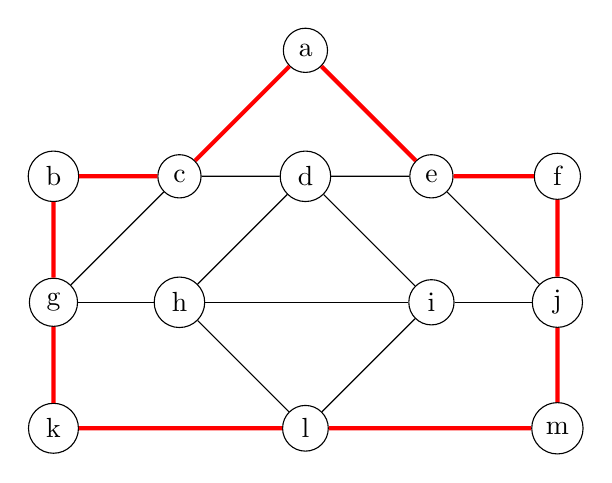
\begin{tikzpicture}[scale=0.8]
        \node[circle,draw] (a) at (0,4) {a};
        \node[circle,draw] (b) at (-4,2) {b};
        \node[circle,draw] (c) at (-2,2) {c};
        \node[circle,draw] (d) at (0,2) {d};
        \node[circle,draw] (e) at (2,2) {e};
        \node[circle,draw] (f) at (4,2) {f};
        \node[circle,draw] (g) at (-4,0) {g};
        \node[circle,draw] (h) at (-2,0) {h};
        \node[circle,draw] (i) at (2,0) {i};
        \node[circle,draw] (j) at (4,0) {j};
        \node[circle,draw] (k) at (-4,-2) {k};
        \node[circle,draw] (l) at (0,-2) {l};
        \node[circle,draw] (m) at (4,-2) {m};
        \draw (j) -- (e) edge[red, line width=1.5pt] (a);
        \draw (g) -- (c) edge[red, line width=1.5pt] (a);
        \draw (d) -- (h) -- (l) -- (i) -- (d);
        \draw (b) edge[red, line width=1.5pt] (g) ;
        \draw (g) edge[red, line width=1.5pt] (k);
        \draw (f) edge[red, line width=1.5pt] (j);
        \draw (j) edge[red, line width=1.5pt] (m);
        \draw (d) -- (c) edge[red, line width=1.5pt] (b);
        \draw (d) -- (e) edge[red, line width=1.5pt] (f);
        \draw (g) -- (h) -- (i) -- (j);
        \draw (k) edge[red, line width=1.5pt] (l);
        \draw (l) edge[red, line width=1.5pt] (m);
    \end{tikzpicture}

    \item \textbf{Inner Vertices:} The vertices which are not visited in the outer loop are \( d \), \( h \) and \( i \). To form a Hamiltonian circuit, we must also visit these inner vertices exactly once.
    
    \item \textbf{Revisiting Vertices:} The challenge arises when we try to connect the outer loop with the inner vertices without revisiting any vertex. Due to the connectivity of graph \( G \), it is not possible to visit all inner vertices without revisiting at least one vertex, breaking the condition for a Hamiltonian circuit.
\end{itemize}

Based on the structure of the graph \( G \) and the analysis above, we can conclude that there is no Hamiltonian circuit in graph \( G \). The inability to connect the outer loop with the inner vertices without revisiting a vertex confirms the absence of a Hamiltonian circuit in this graph.


\subsection*{d)}

Yes there is a Hamilton path in G: \(  b - c - a - e - f - j - m - l - i-d-h-g-k \)

\subsection*{e)}

To determine the chromatic number \( \chi(G) \) of the graph \( G \):

\begin{enumerate}
    \item \textbf{Subgraph Analysis:} Consider the subgraph of \( G \) with the maximum size that forms a complete graph, \( K_3 \) (a triangle). This subgraph consists of vertices \( a \), \( b \), and \( c \). Given that \( K_3 \) requires 3 different colors to ensure no adjacent vertices share the same color, we know that at least 3 colors are necessary.
    
    \item \textbf{Degree and Chromatic Number Relation:} There's a relationship between the maximum degree of a graph and its chromatic number. Specifically, for a graph with maximum degree \( k \), it is \( (k+1) \)-colorable. In \( G \), the maximum degree is 4. Hence, by this relationship, \( G \) is \( (4+1) \)-colorable, implying \( G \) is 5-colorable.
    
    \item \textbf{Narrowing Down the Options:} Given the insights from the subgraph and the degree-chromatic number relationship, we know that \( 3 \leq \chi(G) \leq 5 \). To find the exact chromatic number, we can attempt to color the graph with 3 colors.
    
    \item \textbf{Verification:} By trying to color the graph \( G \) using only 3 colors, we can verify if it's possible to ensure no adjacent vertices share the same color. If successful, then \( \chi(G) = 3 \). If not, then \( \chi(G) \) would be 4 or 5.
\end{enumerate}

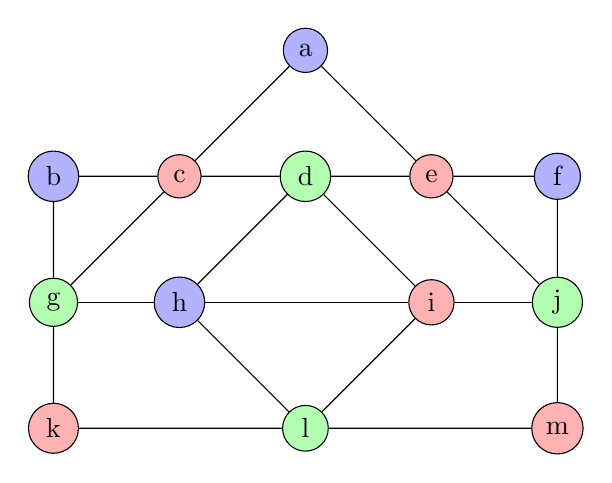
\begin{tikzpicture}[scale=0.8]
    \node[circle,draw,fill=blue!30] (a) at (0,4) {a};
    \node[circle,draw,fill=blue!30] (b) at (-4,2) {b};
    \node[circle,draw,fill=red!30] (c) at (-2,2) {c};
    \node[circle,draw,fill=green!30] (d) at (0,2) {d};
    \node[circle,draw,fill=red!30] (e) at (2,2) {e};
    \node[circle,draw,fill=blue!30] (f) at (4,2) {f};
    \node[circle,draw,fill=green!30] (g) at (-4,0) {g};
    \node[circle,draw,fill=blue!30] (h) at (-2,0) {h};
    \node[circle,draw,fill=red!30] (i) at (2,0) {i};
    \node[circle,draw,fill=green!30] (j) at (4,0) {j};
    \node[circle,draw,fill=red!30] (k) at (-4,-2) {k};
    \node[circle,draw,fill=green!30] (l) at (0,-2) {l};
    \node[circle,draw,fill=red!30] (m) at (4,-2) {m};
    \draw (a) -- (e) -- (j);
    \draw (a) -- (c) -- (g);
    \draw (d) -- (h) -- (l) -- (i) -- (d);
    \draw (b) -- (g) -- (k);
    \draw (f) -- (j) -- (m);
    \draw (b) -- (c) -- (d) -- (e) -- (f);
    \draw (g) -- (h) -- (i) -- (j);
    \draw (k) -- (l) -- (m);
\end{tikzpicture}

\textbf{Conclusion:}

After attempting to color the graph \( G \) with 3 colors, we find that it is indeed possible to do so without any adjacent vertices sharing the same color. Thus, the chromatic number \( \chi(G) \) of the graph \( G \) is 3.


\subsection*{f)}

\textbf{Chromatic Number and Bipartite Graphs:} It's correct that the chromatic number of a bipartite graph is 2. Since \( \chi(G) = 3 \) for \( G \), it confirms that \( G \) cannot be bipartite.

\textbf{Making \( G \) Bipartite:} To make \( G \) bipartite, we would aim to decrease its chromatic number to 2. This can be achieved by removing or "breaking" cycles of odd length in \( G \), as any such cycle in a graph prevents it from being bipartite.

\textbf{Removing \( K_3 \) Subgraphs:} You correctly identified the \( K_3 \) subgraphs in \( G \). To make \( G \) bipartite by removing edges, we would focus on the \( K_3 \) subgraphs.

\begin{itemize}
    \item For \( K_3 \) subgraphs where all vertices are pairwise connected, removing any single edge would suffice.
    
    \item For \( K_3 \) subgraphs where two \( K_3 \) subgraphs share a common edge (forming a 4-clique or \( K_4 \)), removing just one edge would break both \( K_3 \) subgraphs into separate components.
\end{itemize}

Note that we need to create odd cycle.
The steps are so simple:
Select a random node to be the first object in set A. Choose one node to be the first in set B if there are any connected to it. If not, select any other node to be the set B's initial member.

Right now, A and B are our two sets of nodes. Select a node that is not in either set repeatedly. Determine how many edges connect that node to the nodes in A and B. Remove the edges connecting it to nodes in set B and place it in set B if there are further edges connecting it to set A. If not, insert it into set A and remove the edges connecting it to the nodes there.

Thus, \( b-c \), \( e-f \),\( h-i \) are the edges that should be deleted to get bipartite graph.

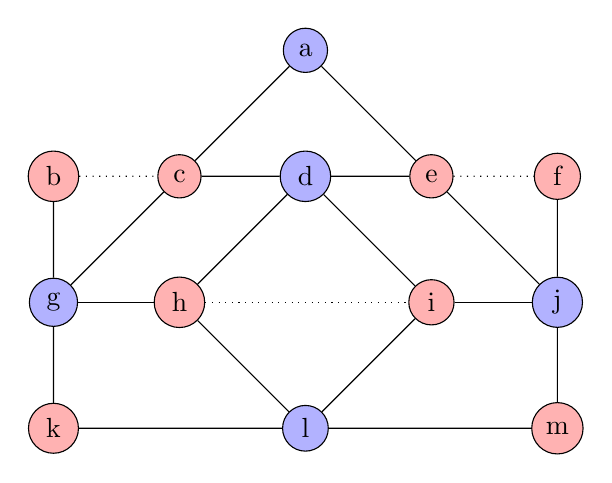
\begin{tikzpicture}[scale=0.8]
    \node[circle,draw,fill=blue!30] (a) at (0,4) {a};
    \node[circle,draw,fill=red!30] (b) at (-4,2) {b};
    \node[circle,draw,fill=red!30] (c) at (-2,2) {c};
    \node[circle,draw,fill=blue!30] (d) at (0,2) {d};
    \node[circle,draw,fill=red!30](e) at (2,2) {e};
    \node[circle,draw,fill=red!30] (f) at (4,2) {f};
    \node[circle,draw,fill=blue!30] (g) at (-4,0) {g};
    \node[circle,draw,fill=red!30] (h) at (-2,0) {h};
    \node[circle,draw,fill=red!30] (i) at (2,0) {i};
    \node[circle,draw,fill=blue!30] (j) at (4,0) {j};
    \node[circle,draw,fill=red!30] (k) at (-4,-2) {k};
    \node[circle,draw,fill=blue!30] (l) at (0,-2) {l};
    \node[circle,draw,fill=red!30] (m) at (4,-2) {m};
    \draw (a) -- (e) -- (j);
    \draw (a) -- (c) -- (g);
    \draw (d) -- (h) -- (l) -- (i) -- (d);
    \draw (b) -- (g) -- (k);
    \draw (f) -- (j) -- (m);
    \draw[dotted] (b) -- (c); 
    \draw (c)-- (d) -- (e);
    \draw[dotted] (e) -- (f);
    \draw (g) -- (h) ;
    \draw[dotted] (h) -- (i);cxxx
    \draw (i) -- (j);
    \draw (k) -- (l) -- (m);
\end{tikzpicture}

\subsection*{g)}

Given the graph \( G \) with chromatic number \( \chi(G) = 3 \), it indicates that no set of four vertices in \( G \) can form a complete subgraph \( K_4 \) since a \( K_4 \) would require 4 distinct colors.

Upon examining the graph:

\begin{enumerate}
    \item Vertices \( d \), \( h \), and \( i \) form a complete subgraph \( K_3 \).
\end{enumerate}

To introduce a complete subgraph \( K_4 \) into \( G \), we need to add a vertex connected to \( d \), \( h \), \( i \), and \( l \).

The edge between vertices \( d \) and \( l \) can be added to \( G \) to ensure that the vertices \( d \), \( h \), \( i \), and \( l \) together form a complete subgraph \( K_4 \).

Thus, to incorporate a complete subgraph \( K_4 \) into \( G \), the edge connecting \( d \) and \( l \) should be added.


\section*{Answer 2}



\section*{Answer 3}

\subsection*{a)}

\subsection*{b)}

\section*{Answer 4}

\subsection*{a)}

\subsection*{b)}

\subsection*{c)}


\section*{Answer 5}

\subsection*{a)}

\subsection*{b)}

\subsection*{c)}

\end{document}
